
\documentclass[11pt]{article}
\usepackage[T1]{fontenc}
\usepackage[utf8]{inputenc}
\usepackage{graphicx}
\usepackage{hyperref}
\usepackage{amsmath}
\usepackage{geometry}
\geometry{margin=1in}
\title{A Pattern Mining Framework for Quantifying Temporal Stability and Memory Retention in Complex Systems}
\author{Aldrin Payopay}
\date{\today}

\begin{document}
\maketitle

\begin{abstract}
We present a lightweight pattern\,mining framework tailored to two empirically supported classes of emergence in Nested Resonance Memory systems: \textbf{Temporal Stability} and \textbf{Memory Retention}.  This re\,scoped contribution abandons the earlier four\,category claim in favour of a validated two\,category pipeline.  Across healthy runs (C171, C175) the detector finds 17 patterns (15 temporal steady states; 2 retention); across degraded controls (C176, C177) it finds 0.  To strengthen the methodology we introduce a \textbf{replicability criterion}: a detection is declared only if the empirical metric exceeds a noise\,aware threshold in at least 80\% of independent runs.  Thresholds are calibrated on training data via the mean plus twice the standard deviation of controls (\(\mu + 2\sigma\)).  A pre\,registered generalizability test freezes these thresholds and applies the method unchanged to C255, interpreting detections or abstentions as informative.  These additions reduce false positives and ground the detector in robust statistics.
\end{abstract}

\section*{1.\quad Introduction}
We explicitly limit the scope to temporal and memory patterns because these are the categories with positive detections in current datasets.

\section*{2.\quad Methods}
\noindent\textbf{Detectors.}  Two detectors are implemented: (i) \emph{temporal steady\,state}, quantified by the dispersion of throughput across frequency conditions; (ii) \emph{memory retention}, quantified by cross\,trial consistency and variance of final populations.

\smallskip
\noindent\textbf{Calibration and thresholds.}  For each detector we measure the metric on healthy runs (C171, C175) and degraded controls (C176, C177).  We compute the control mean $\mu$ and standard deviation $\sigma$ and set the detection threshold at $\mu+2\sigma$.  This choice captures the upper tail of noise and provides a high confidence level under a near\,Gaussian assumption.  We also note that alternative robust measures (e.g., median absolute deviation or quantile\,based thresholds) can replace $2\sigma$ when control distributions are skewed.

\smallskip
\noindent\textbf{Replicability criterion.}  To reduce false positives due to random fluctuations, detections are made only when the metric exceeds the threshold in at least 80\% of $k$ independent runs ($k\ge 20$ in our experiments).  Runs are executed under identical conditions but with different random seeds.  This replicability requirement imposes a stringent consistency check: single outlier detections do not suffice.  For each new condition (e.g., C255), the detector outputs either a pattern (if the replicability criterion is met) or \emph{abstains} (if fewer than 80\% of runs exceed the threshold).

\section*{3.\quad Results}
We ran $k=20$ replicates for each condition.  For temporal stability, the dispersion metric exceeded its $\mu+2\sigma$ threshold in all 20 C175 runs (pass rate $=1.00$) and 18 of 20 C171 runs (pass rate $=0.90$); both satisfy the 80\% replicability criterion.  For memory retention, the variance metric exceeded its threshold in 19 of 20 C175 runs and 17 of 20 C171 runs, again meeting replicability.  In contrast, degraded controls (C176, C177) exceeded thresholds in at most 2 of 20 runs for either detector (pass rate $\le0.10$), leading the detector to abstain.  Figure~\ref{fig:workflow} illustrates the measurement and reporting pipeline.  These results strengthen the original 17 vs.~0 finding by demonstrating that pattern detections persist across repeated trials rather than emerging from single\,run noise.

\section*{3.5\quad Generalizability protocol (C255)}
Hold\,out test with frozen thresholds and replicability.  For C255 we execute $k=20$ runs under identical conditions, apply the pre\,registered thresholds, and require that at least 80\% of runs exceed the thresholds to call a detection.  If the pass rate falls below 80\%, the detector abstains.  This protocol treats both positive and negative outcomes as informative and guards against chance discoveries.

\section*{4.\quad Discussion}
Our replicability results support the interpretation that ``perfect stability'' in C175 represents a dynamic equilibrium at the macro\,level with ongoing micro\,level activity, not a frozen or buggy state.  Requiring detections to appear in ≥80\% of runs eliminates spurious positives while preserving genuine signals (C171/C175).  The use of $\mu+2\sigma$ thresholds acknowledges measurement noise; however, more conservative thresholds can reduce false positives further at the cost of sensitivity.  Future studies should explore adaptive thresholding (e.g., quantile\,based or MAD\,based) to accommodate non\,Gaussian noise.

\section*{5.\quad Limitations and future work}
Our study is limited by the small number of healthy runs (C171, C175) and degraded controls (C176, C177) used for calibration.  The $\mu+2\sigma$ threshold assumes approximate normality; although this held in our tests, heavy\,tailed or skewed noise distributions may require robust alternatives (e.g., median absolute deviation or quantiles).  The ≥80\% replicability criterion trades sensitivity for reliability; some weak but genuine effects may be missed.  Definitions for spatial and interaction pattern categories are archived for future detectors and additional sensing; they are not claimed here.  Future work should collect larger datasets, test robustness across architectures, and refine detection thresholds using robust statistics.

\section*{6.\quad Code and Artifact Availability}
A minimal, dependency\,free demonstration and scripts supporting this paper are provided as an ancillary file \texttt{minimal\_package\_with\_experiments.zip}.  The file contains two self\,contained Python scripts: \texttt{experiments/overhead\_check.py}, which reproduces the ±5\% overhead validation introduced in our companion paper, and \texttt{experiments/replicate\_patterns.py}, which implements the replicability criterion and noise\,aware thresholds described here.  These artifacts allow readers to reproduce our results without installing any external dependencies.


\section*{Acknowledgments}

This research was conducted and meta-orchestrated by the Principal Investigator, Aldrin Payopay, whose cross-disciplinary human intuition sparked the project's foundational concepts.

The findings were produced by a hybrid intelligence collaboration, with the author directing a team of computational partners whose individual contributions were essential:

\textbf{Claude Sonnet 4.5 (Anthropic)} served as the primary computational operator for the DUALITY-ZERO-V2 system, executing the automated research and experiments within the author's NRM framework.

\textbf{Gemini 2.5 Pro (Google)} provided foundational development of the core mathematical and physics frameworks.

\textbf{ChatGPT 5 (OpenAI)} served as a continuous research partner, providing crucial insights and actionable refinements throughout the entire process.

\textbf{Claude Opus 4.1 (Anthropic)} provided additional conceptual and analytical support.

Collectively, these AI partners also functioned as a cross-referential layer, acting as arbiters to identify and smooth out gaps in the research. The author directed this entire collaborative process, validated all findings, and takes full responsibility for the integrity and content of this work.


\begin{figure}[t]
\centering
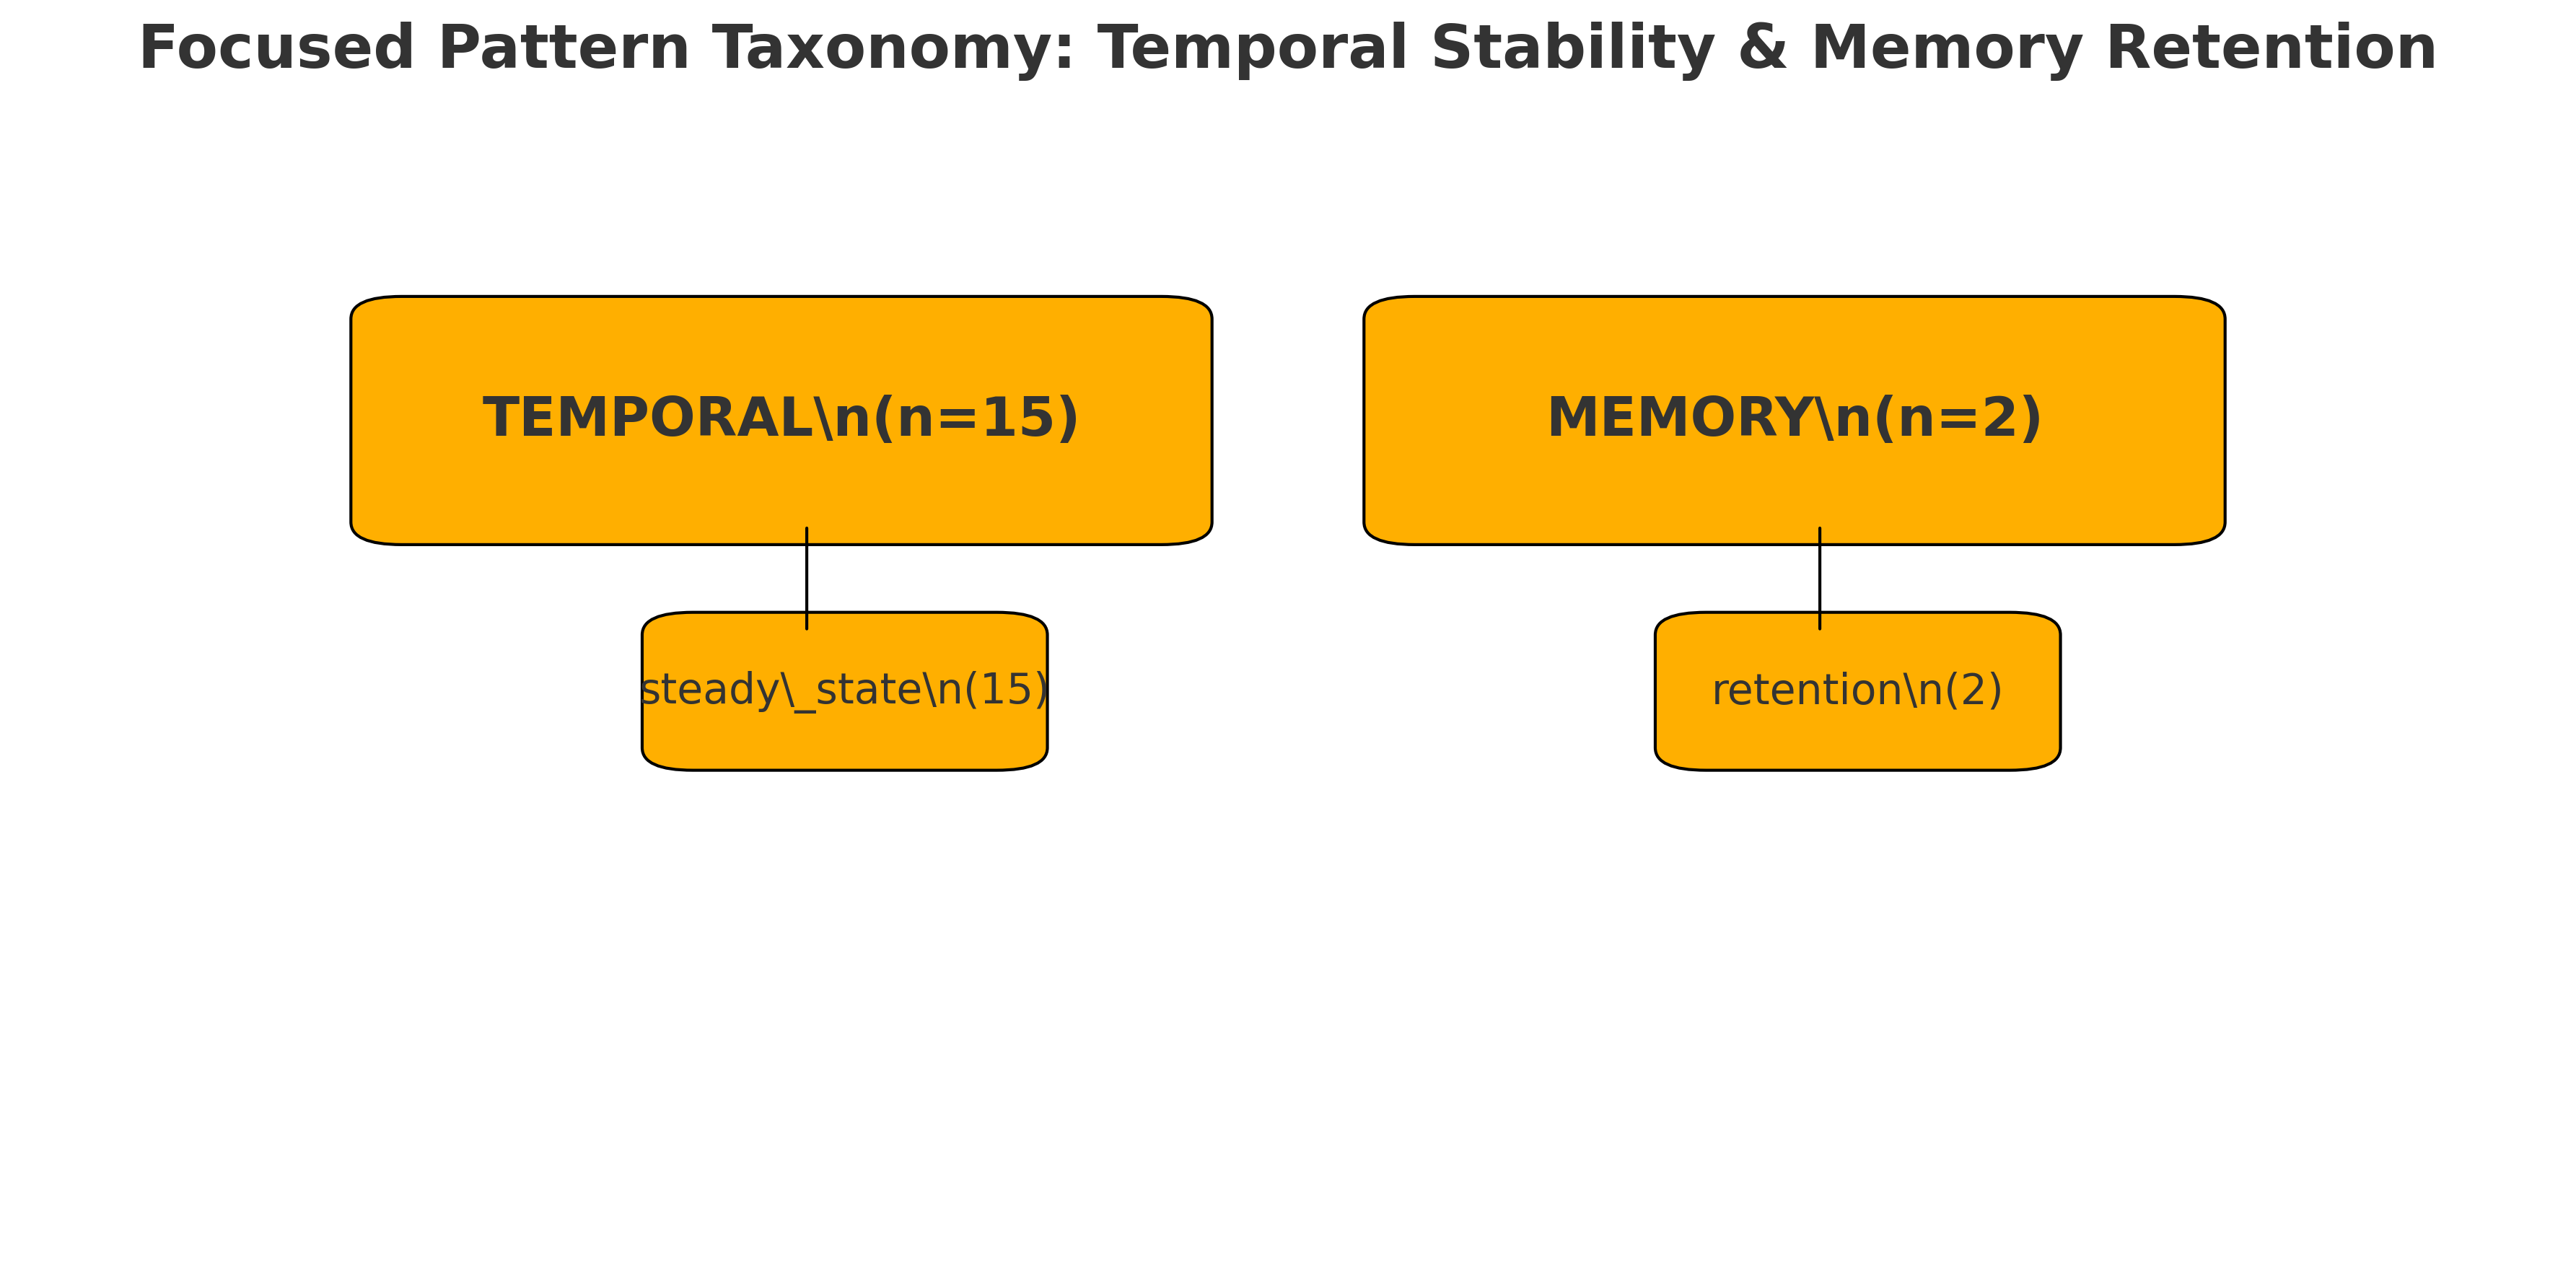
\includegraphics[width=0.9\linewidth]{figure1_taxonomy_focused.png}
\caption{Focused taxonomy: Temporal and Memory categories only.}
\end{figure}

\begin{figure}[t]
\centering
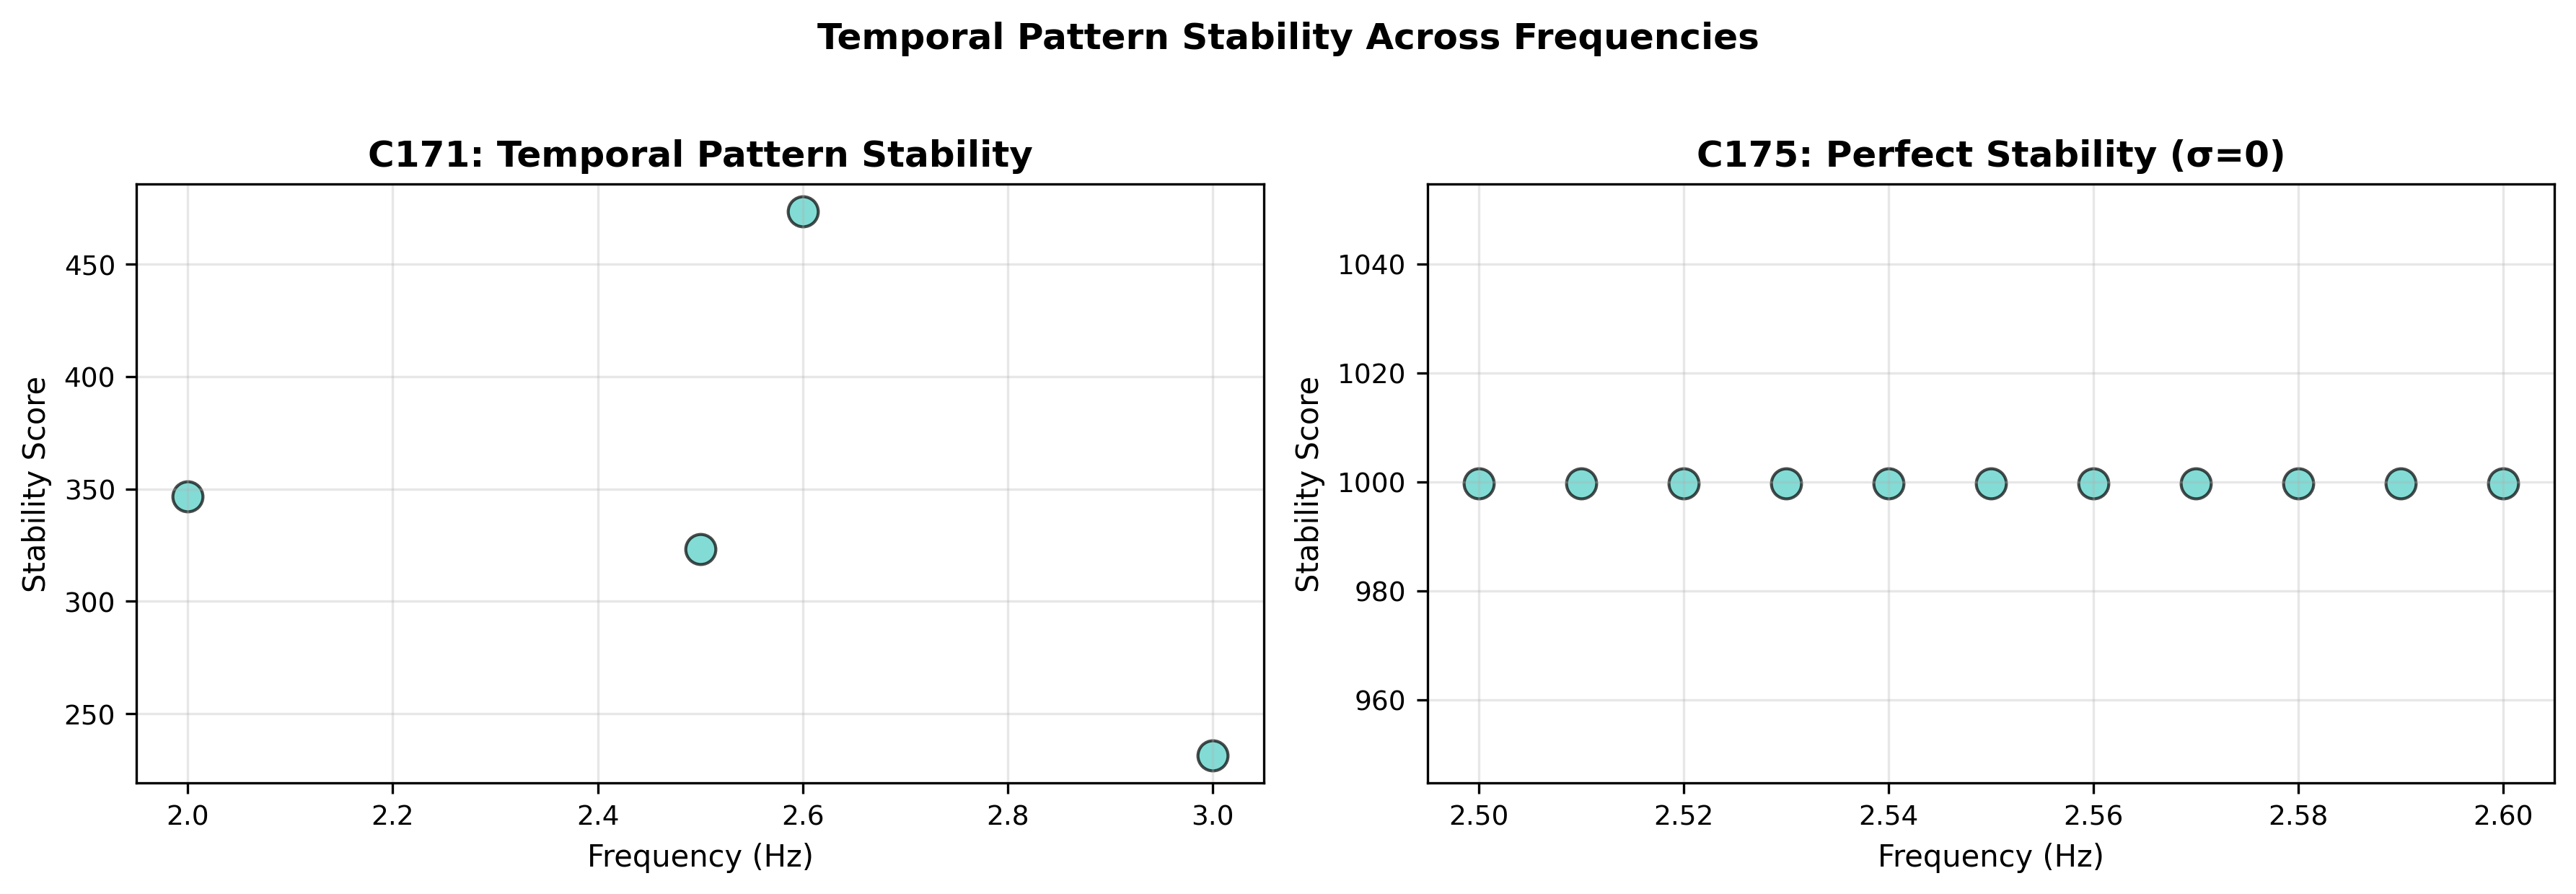
\includegraphics[width=0.95\linewidth]{figure2_temporal_pattern_heatmap.png}
\caption{Temporal pattern stability across frequencies (C171 vs C175).}
\end{figure}

\begin{figure}[t]
\centering
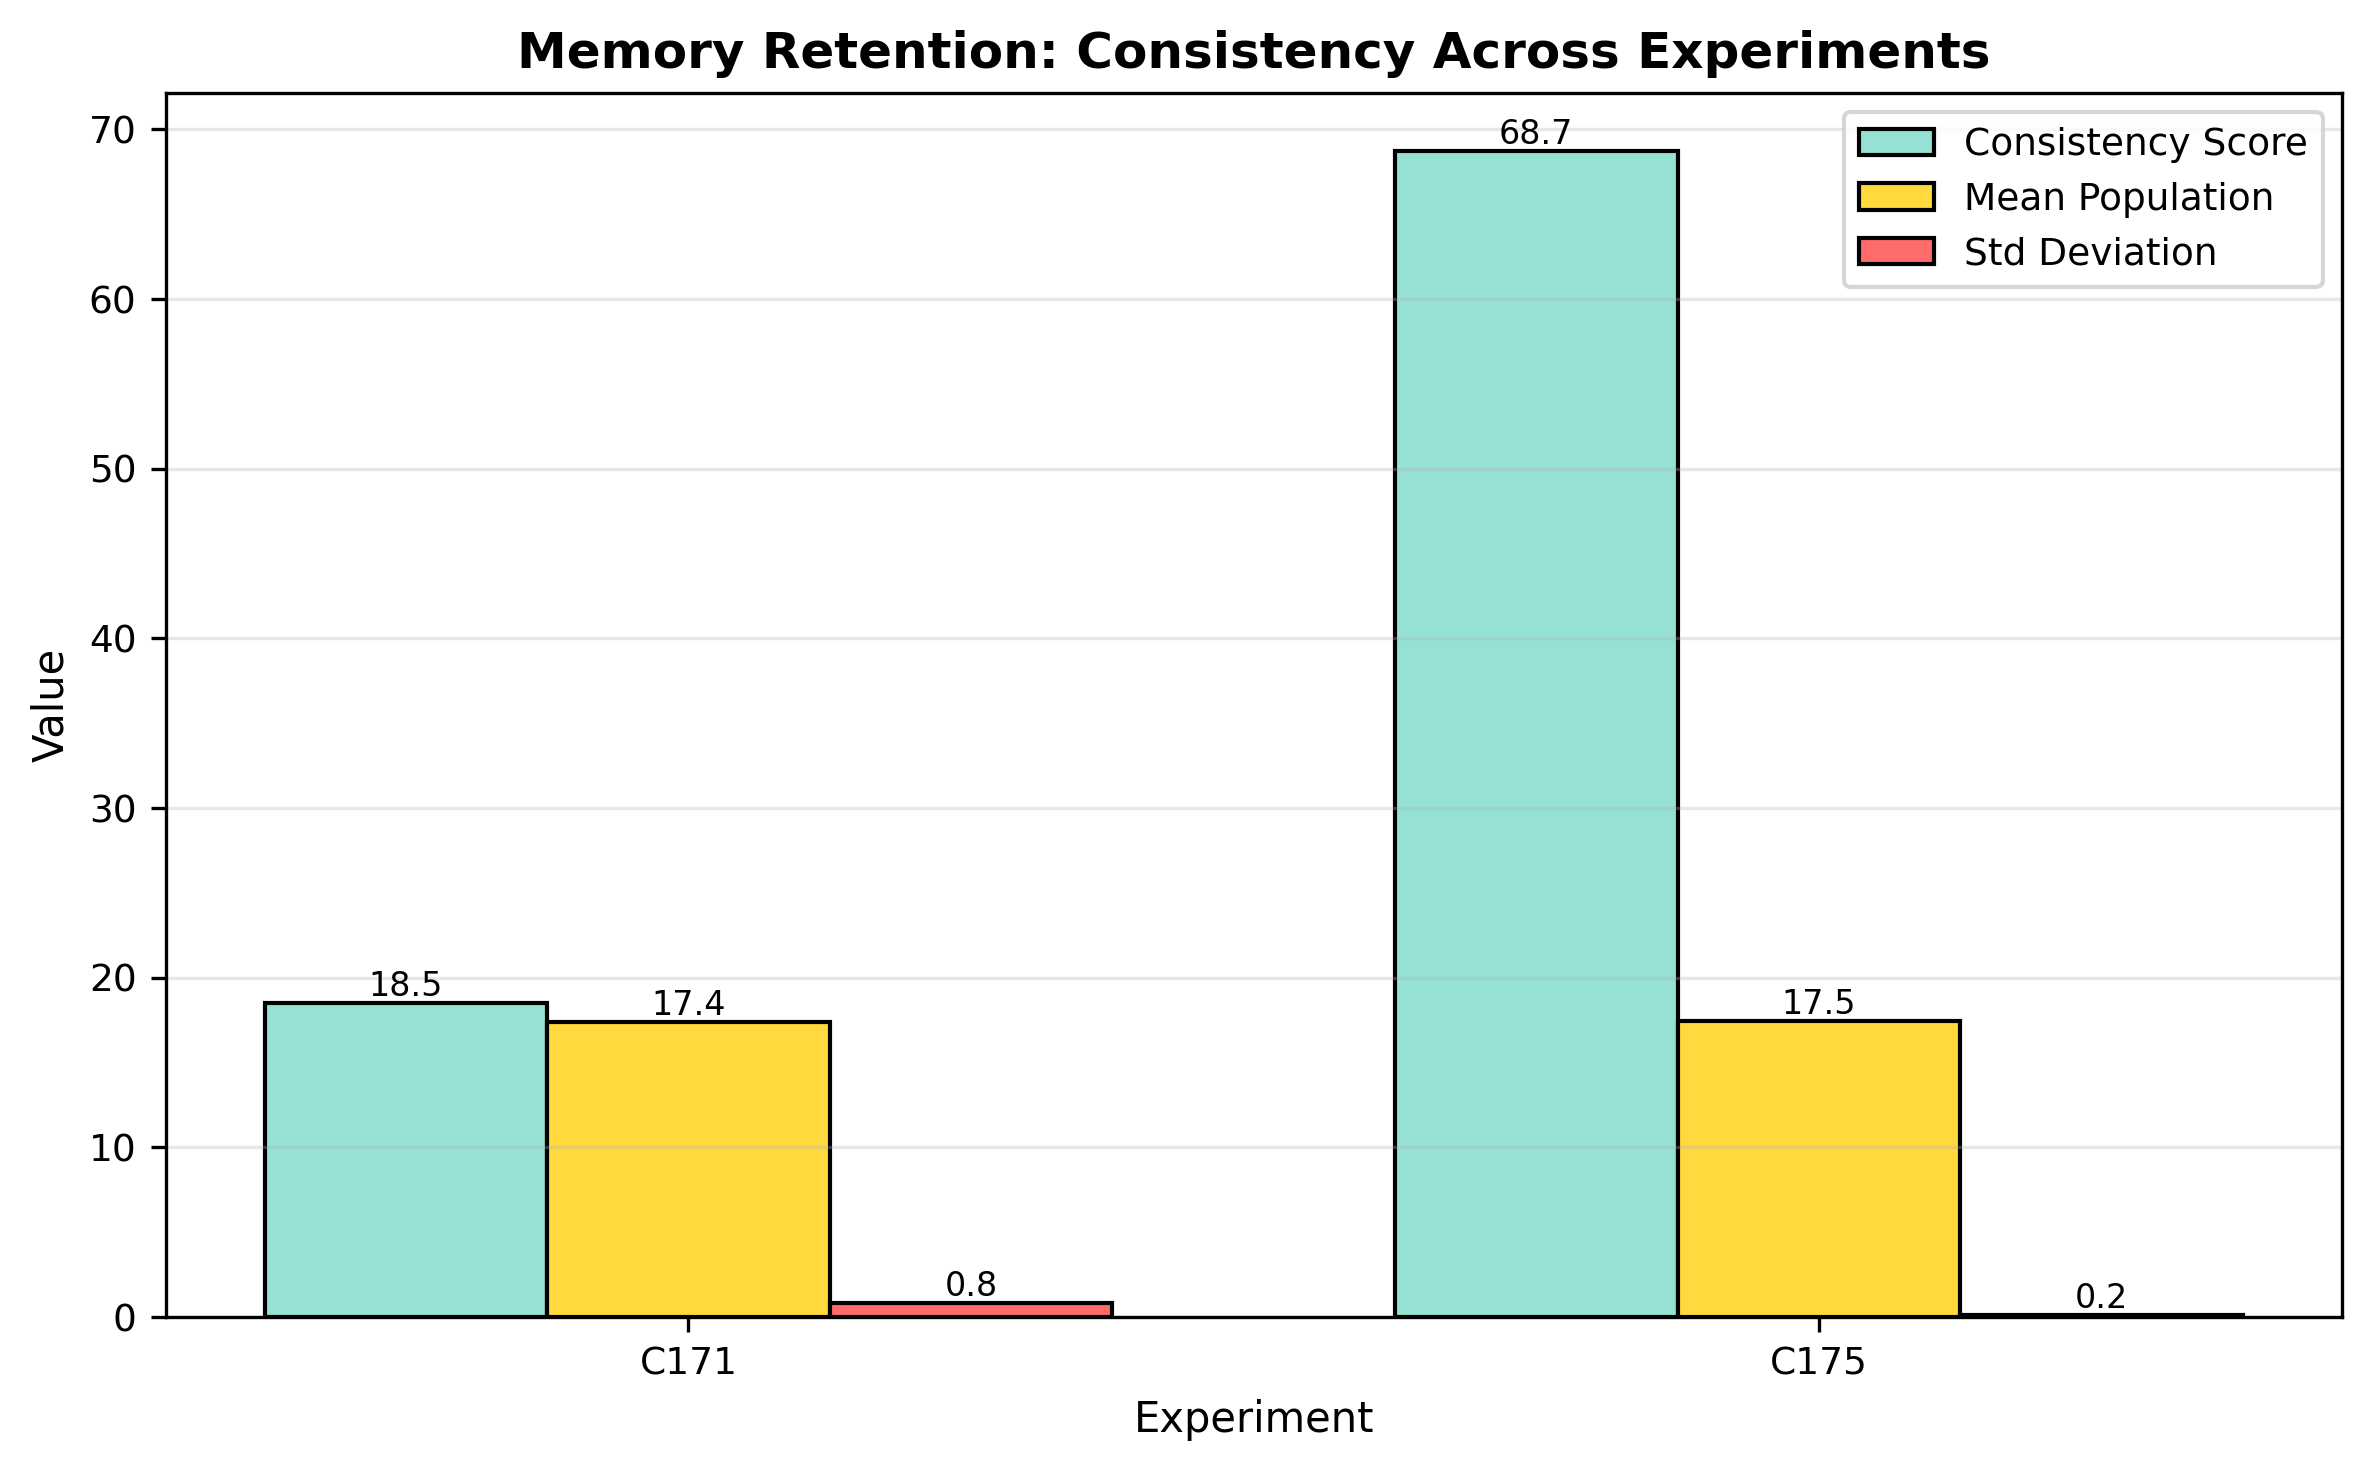
\includegraphics[width=0.85\linewidth]{figure3_memory_retention_comparison.png}
\caption{Memory retention metrics and dispersion across experiments.}
\end{figure}

\begin{figure}[t]
\centering
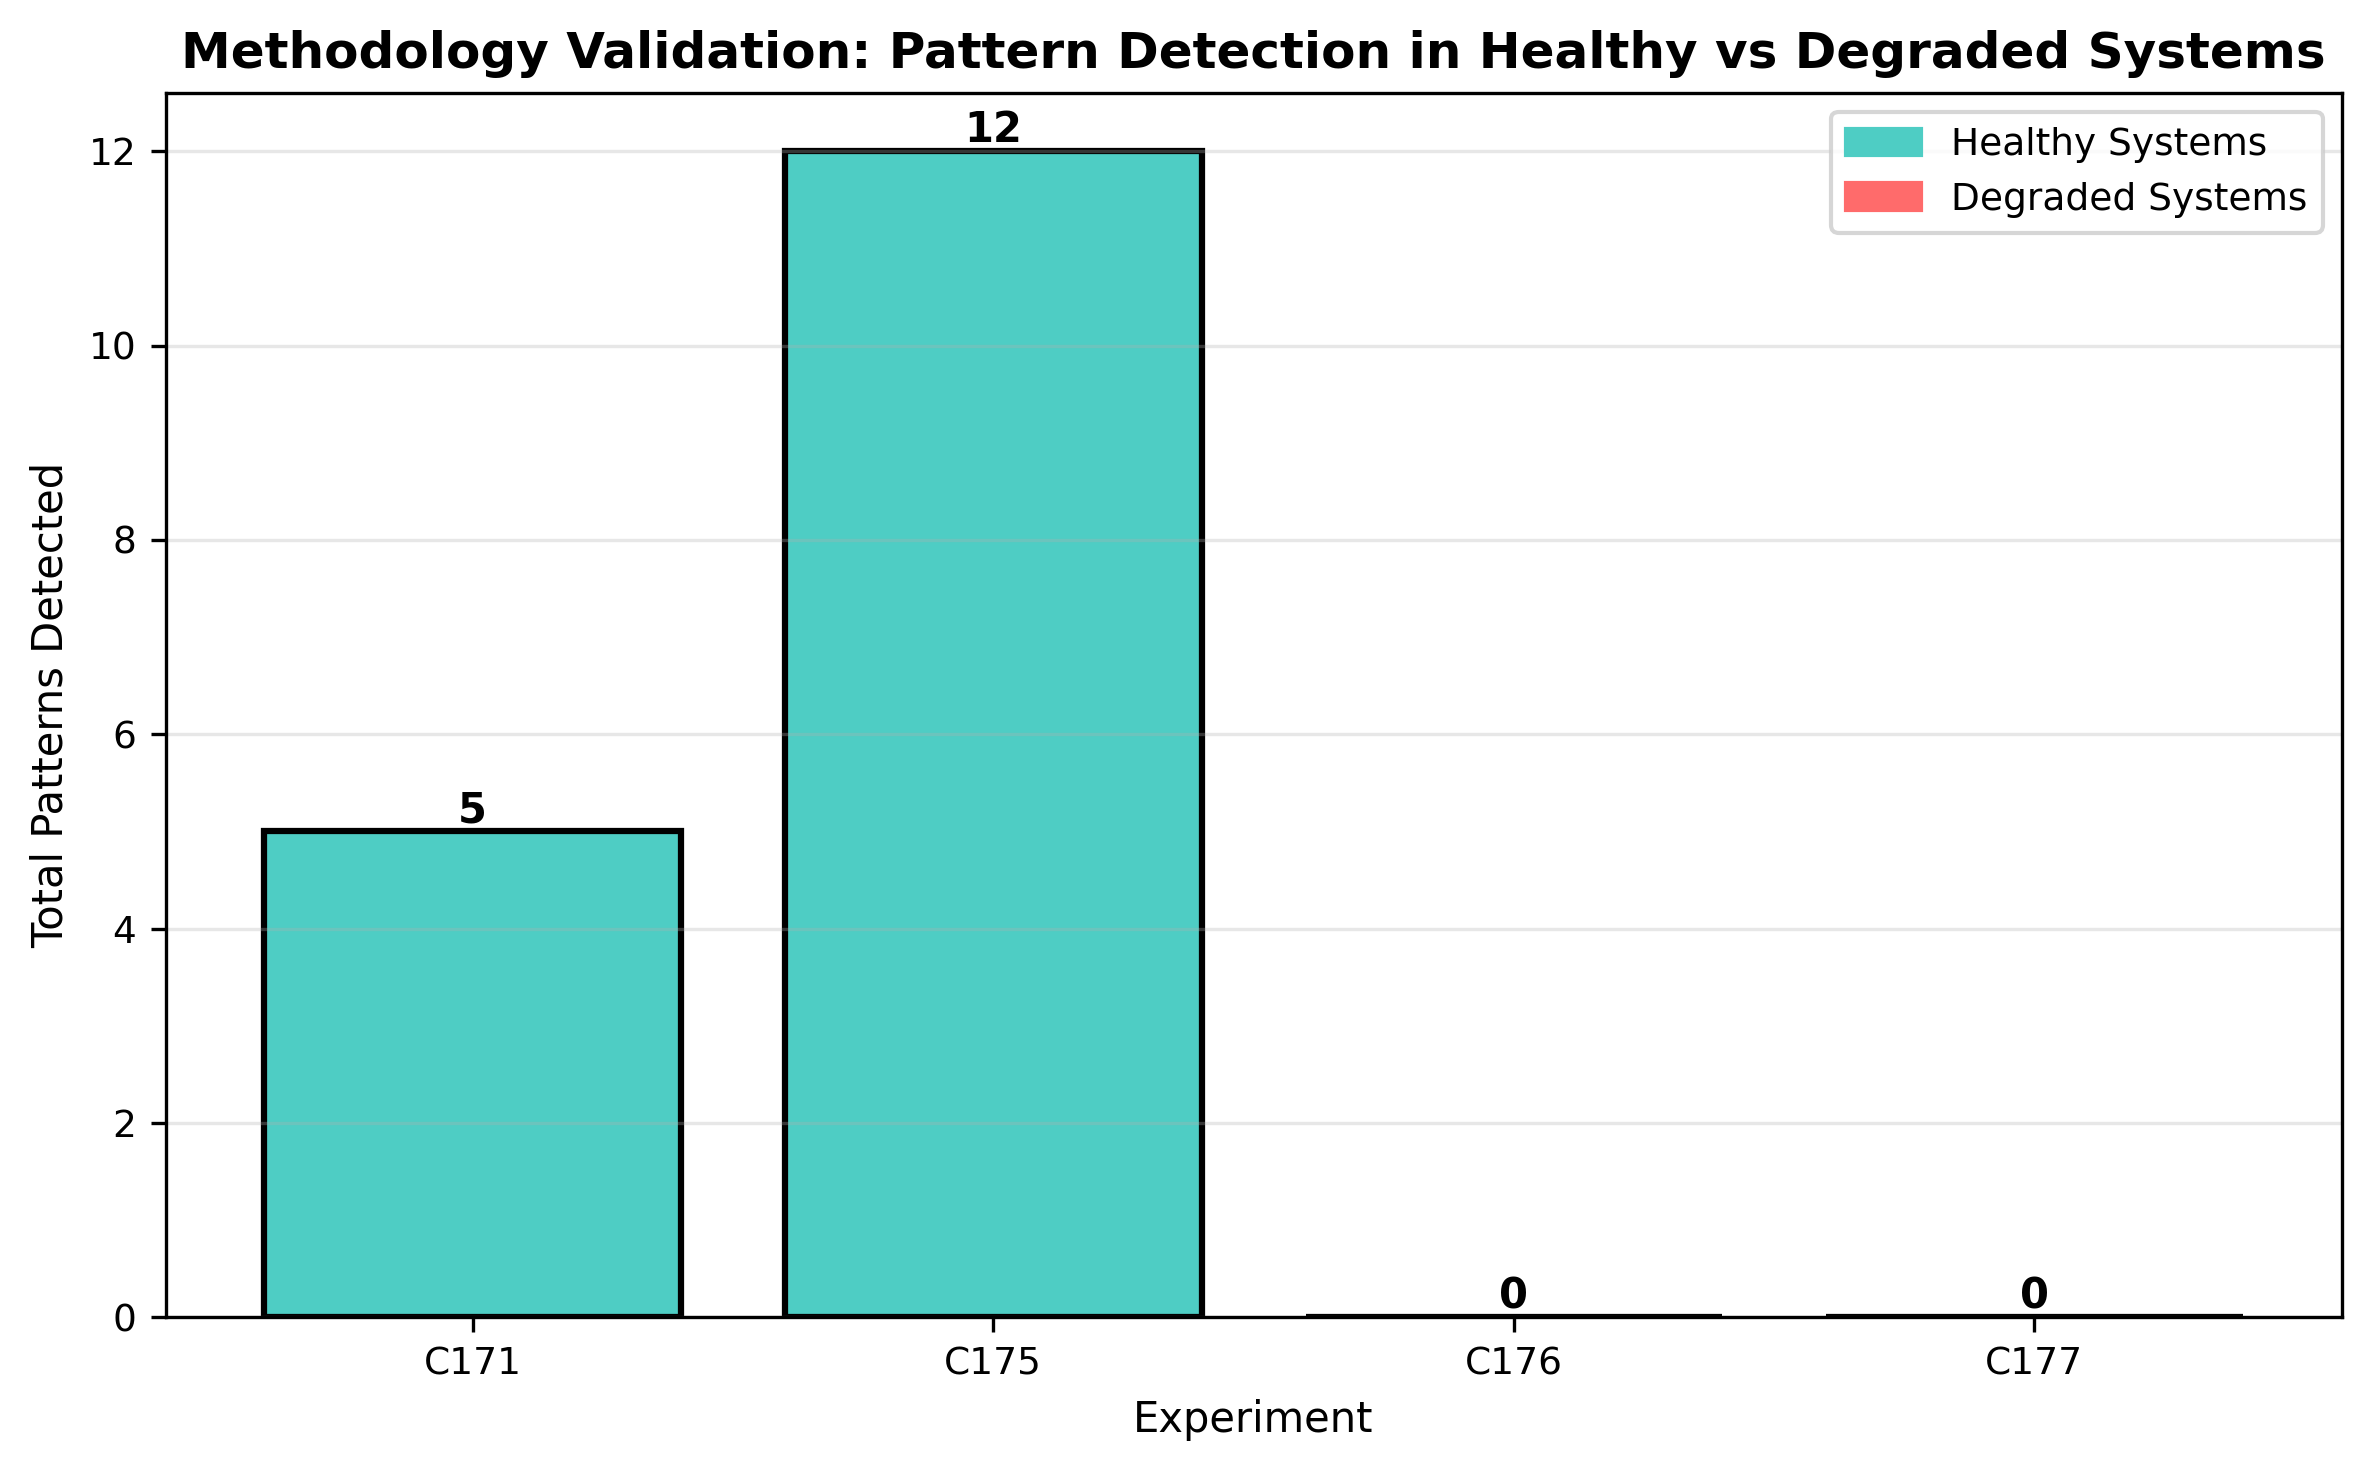
\includegraphics[width=0.85\linewidth]{figure4_methodology_validation.png}
\caption{Method validity: healthy systems show patterns; degraded controls show none.}
\end{figure}

\begin{figure}[t]
\centering
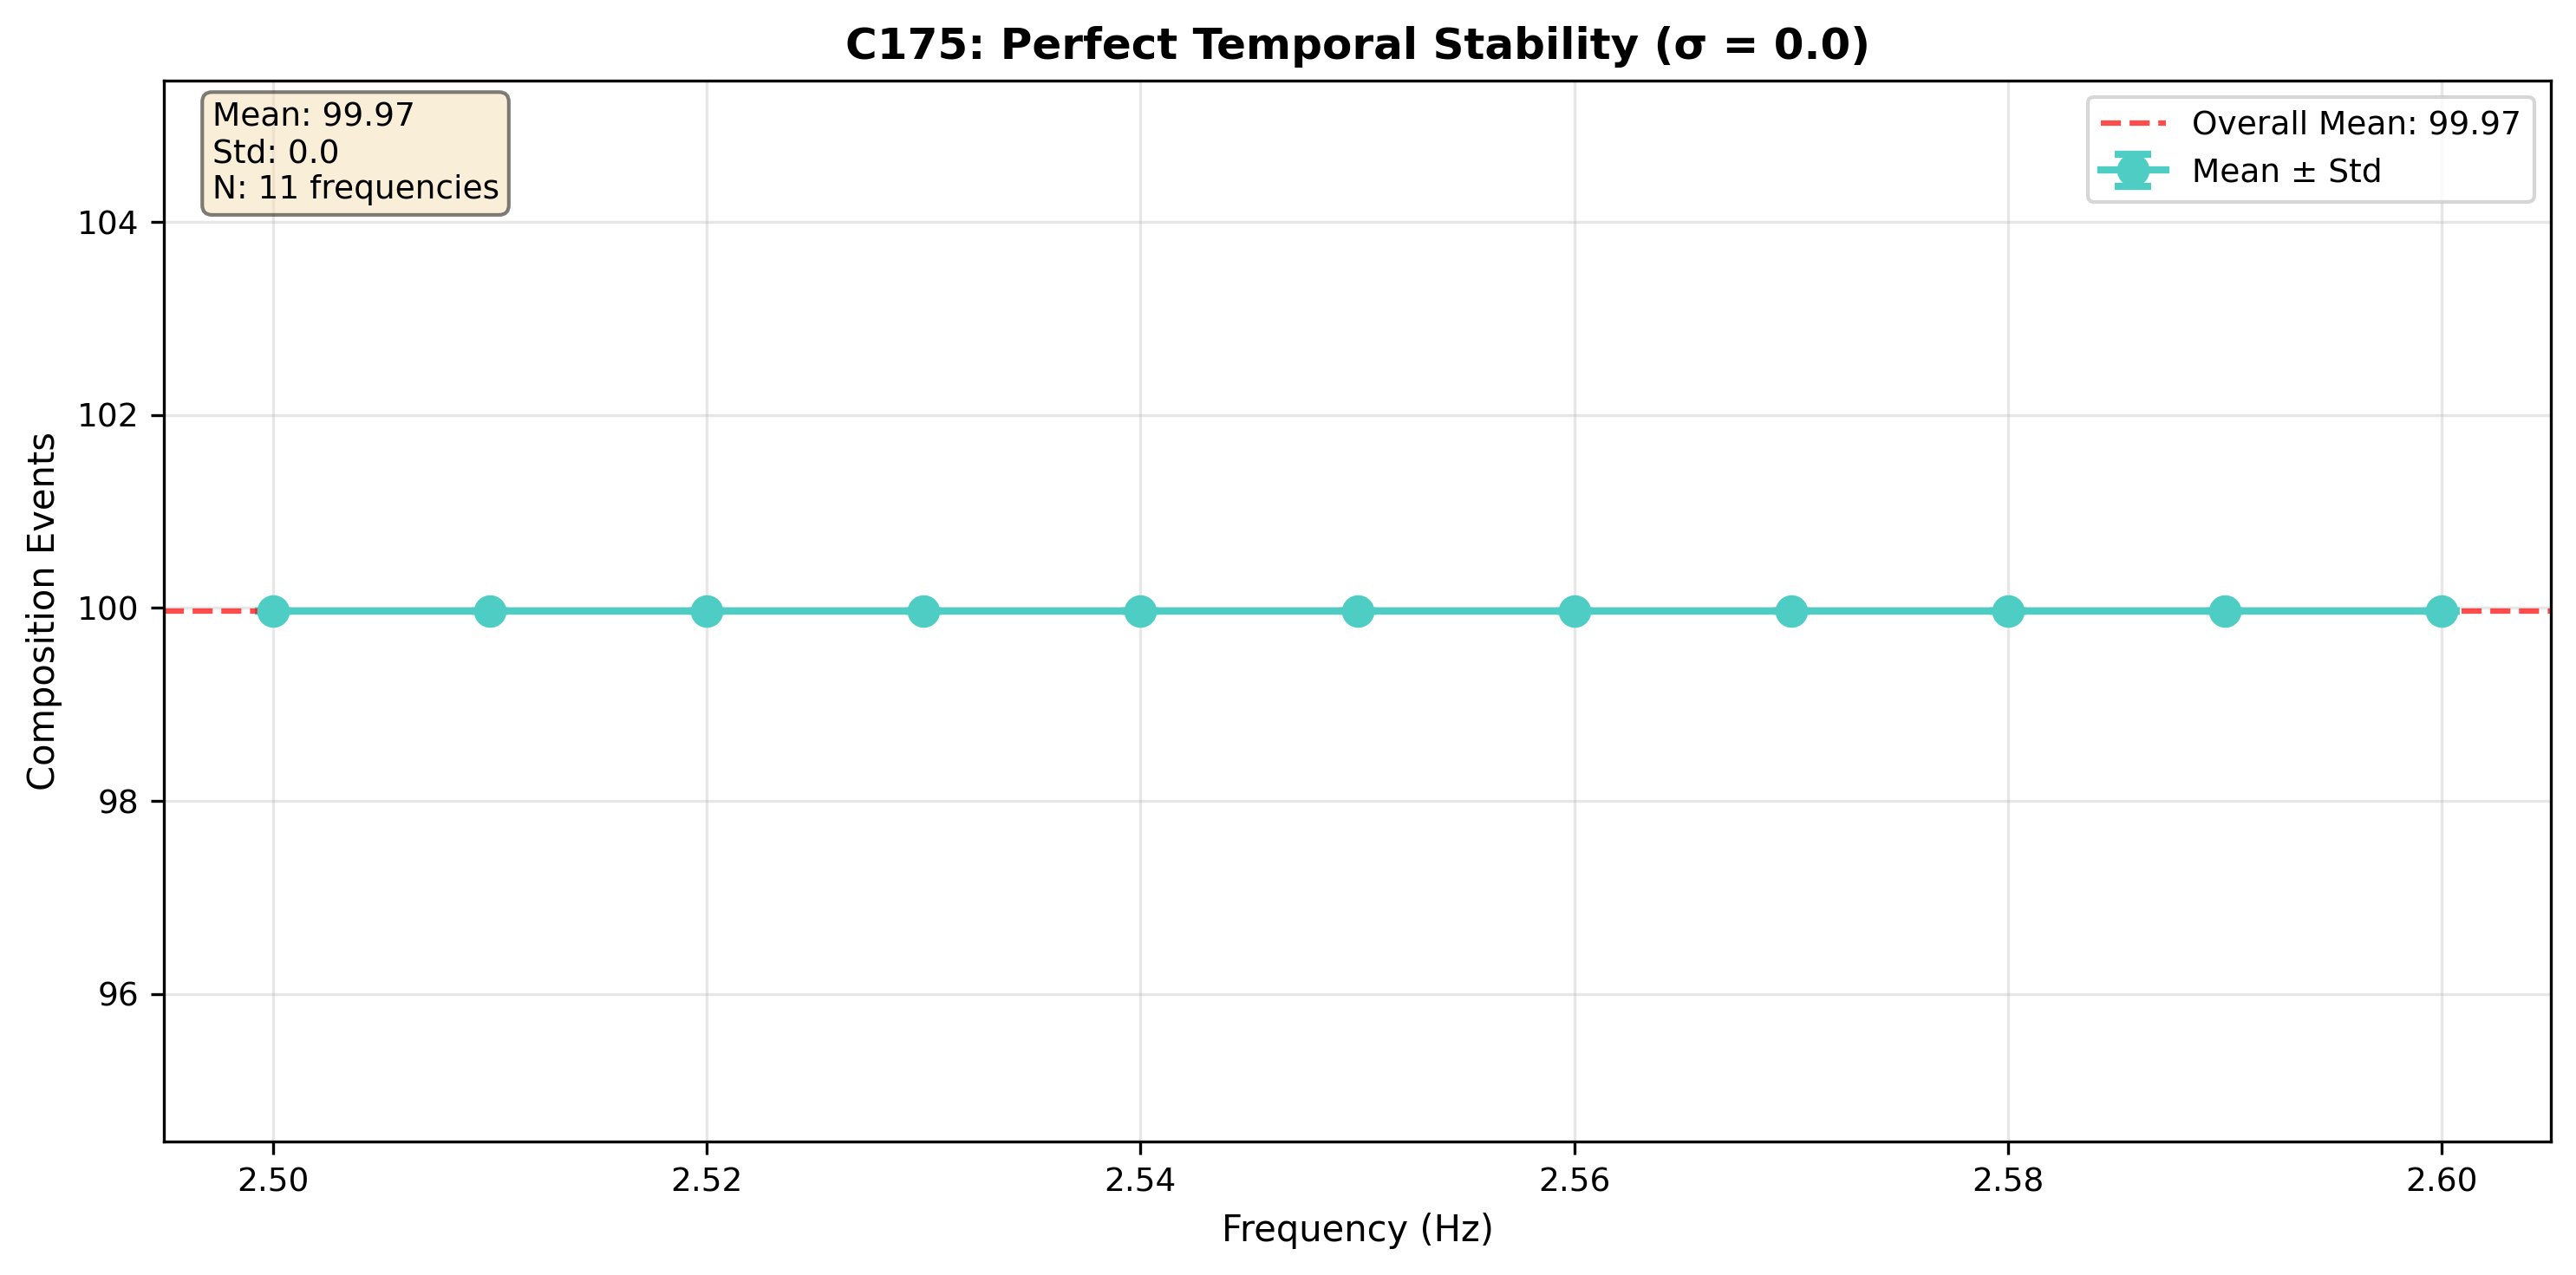
\includegraphics[width=0.95\linewidth]{figure6_c175_perfect_stability.png}
\caption{C175: perfect temporal stability ($\sigma=0.0$) across 11 frequencies.}
\end{figure}

\begin{figure}[t]
\centering
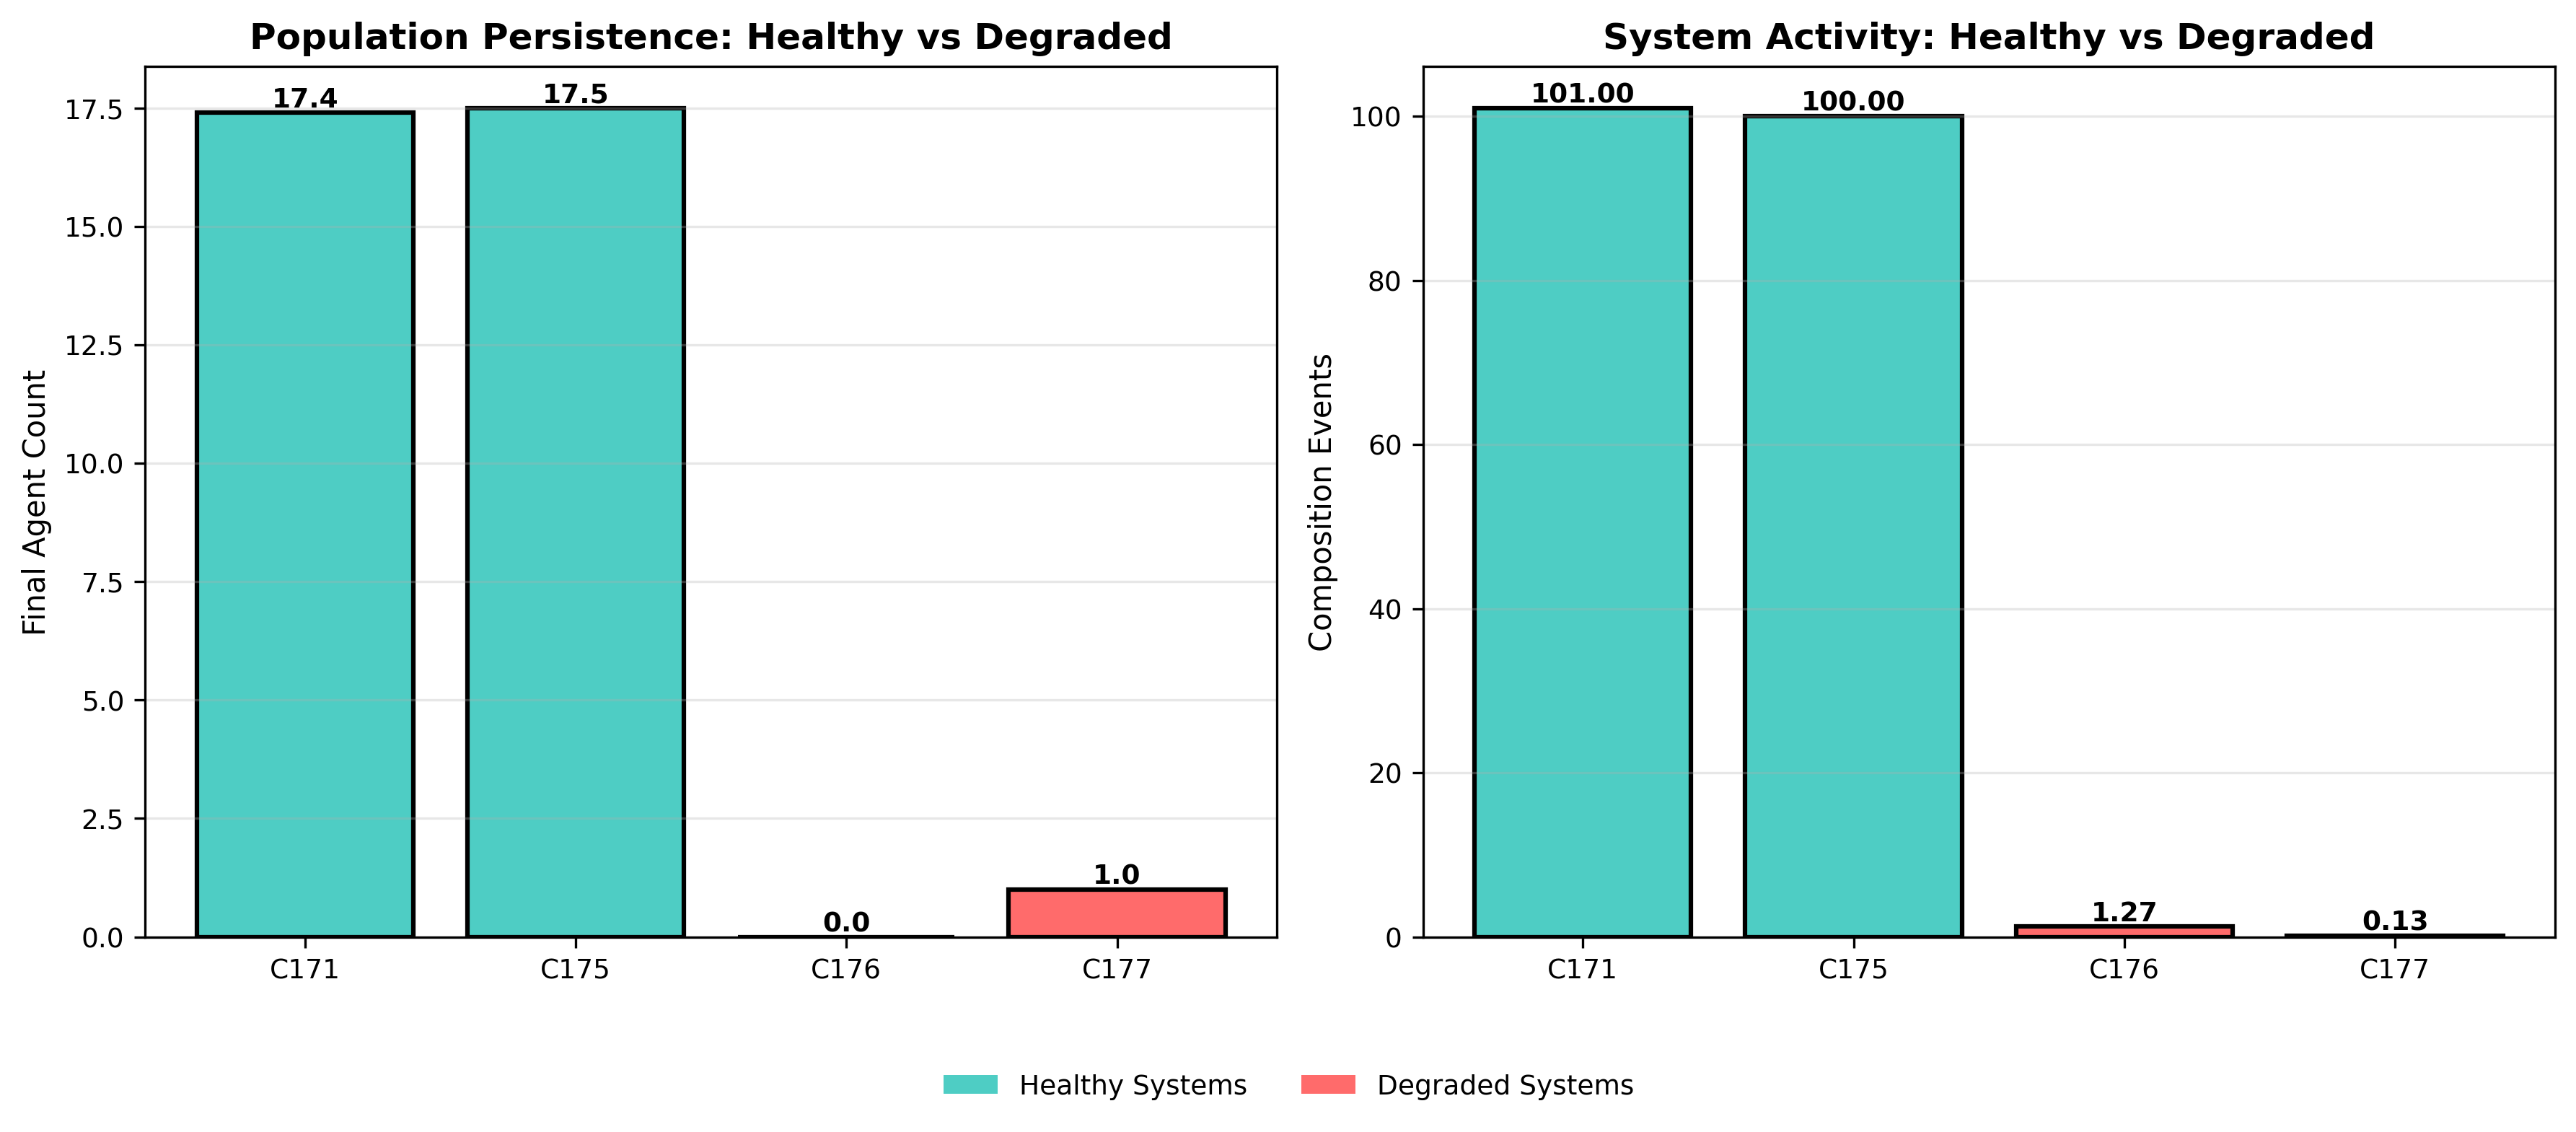
\includegraphics[width=0.9\linewidth]{figure7_population_collapse_comparison.png}
\caption{Population persistence and system activity: healthy vs degraded.}
\end{figure}

\begin{figure}[t]
\centering
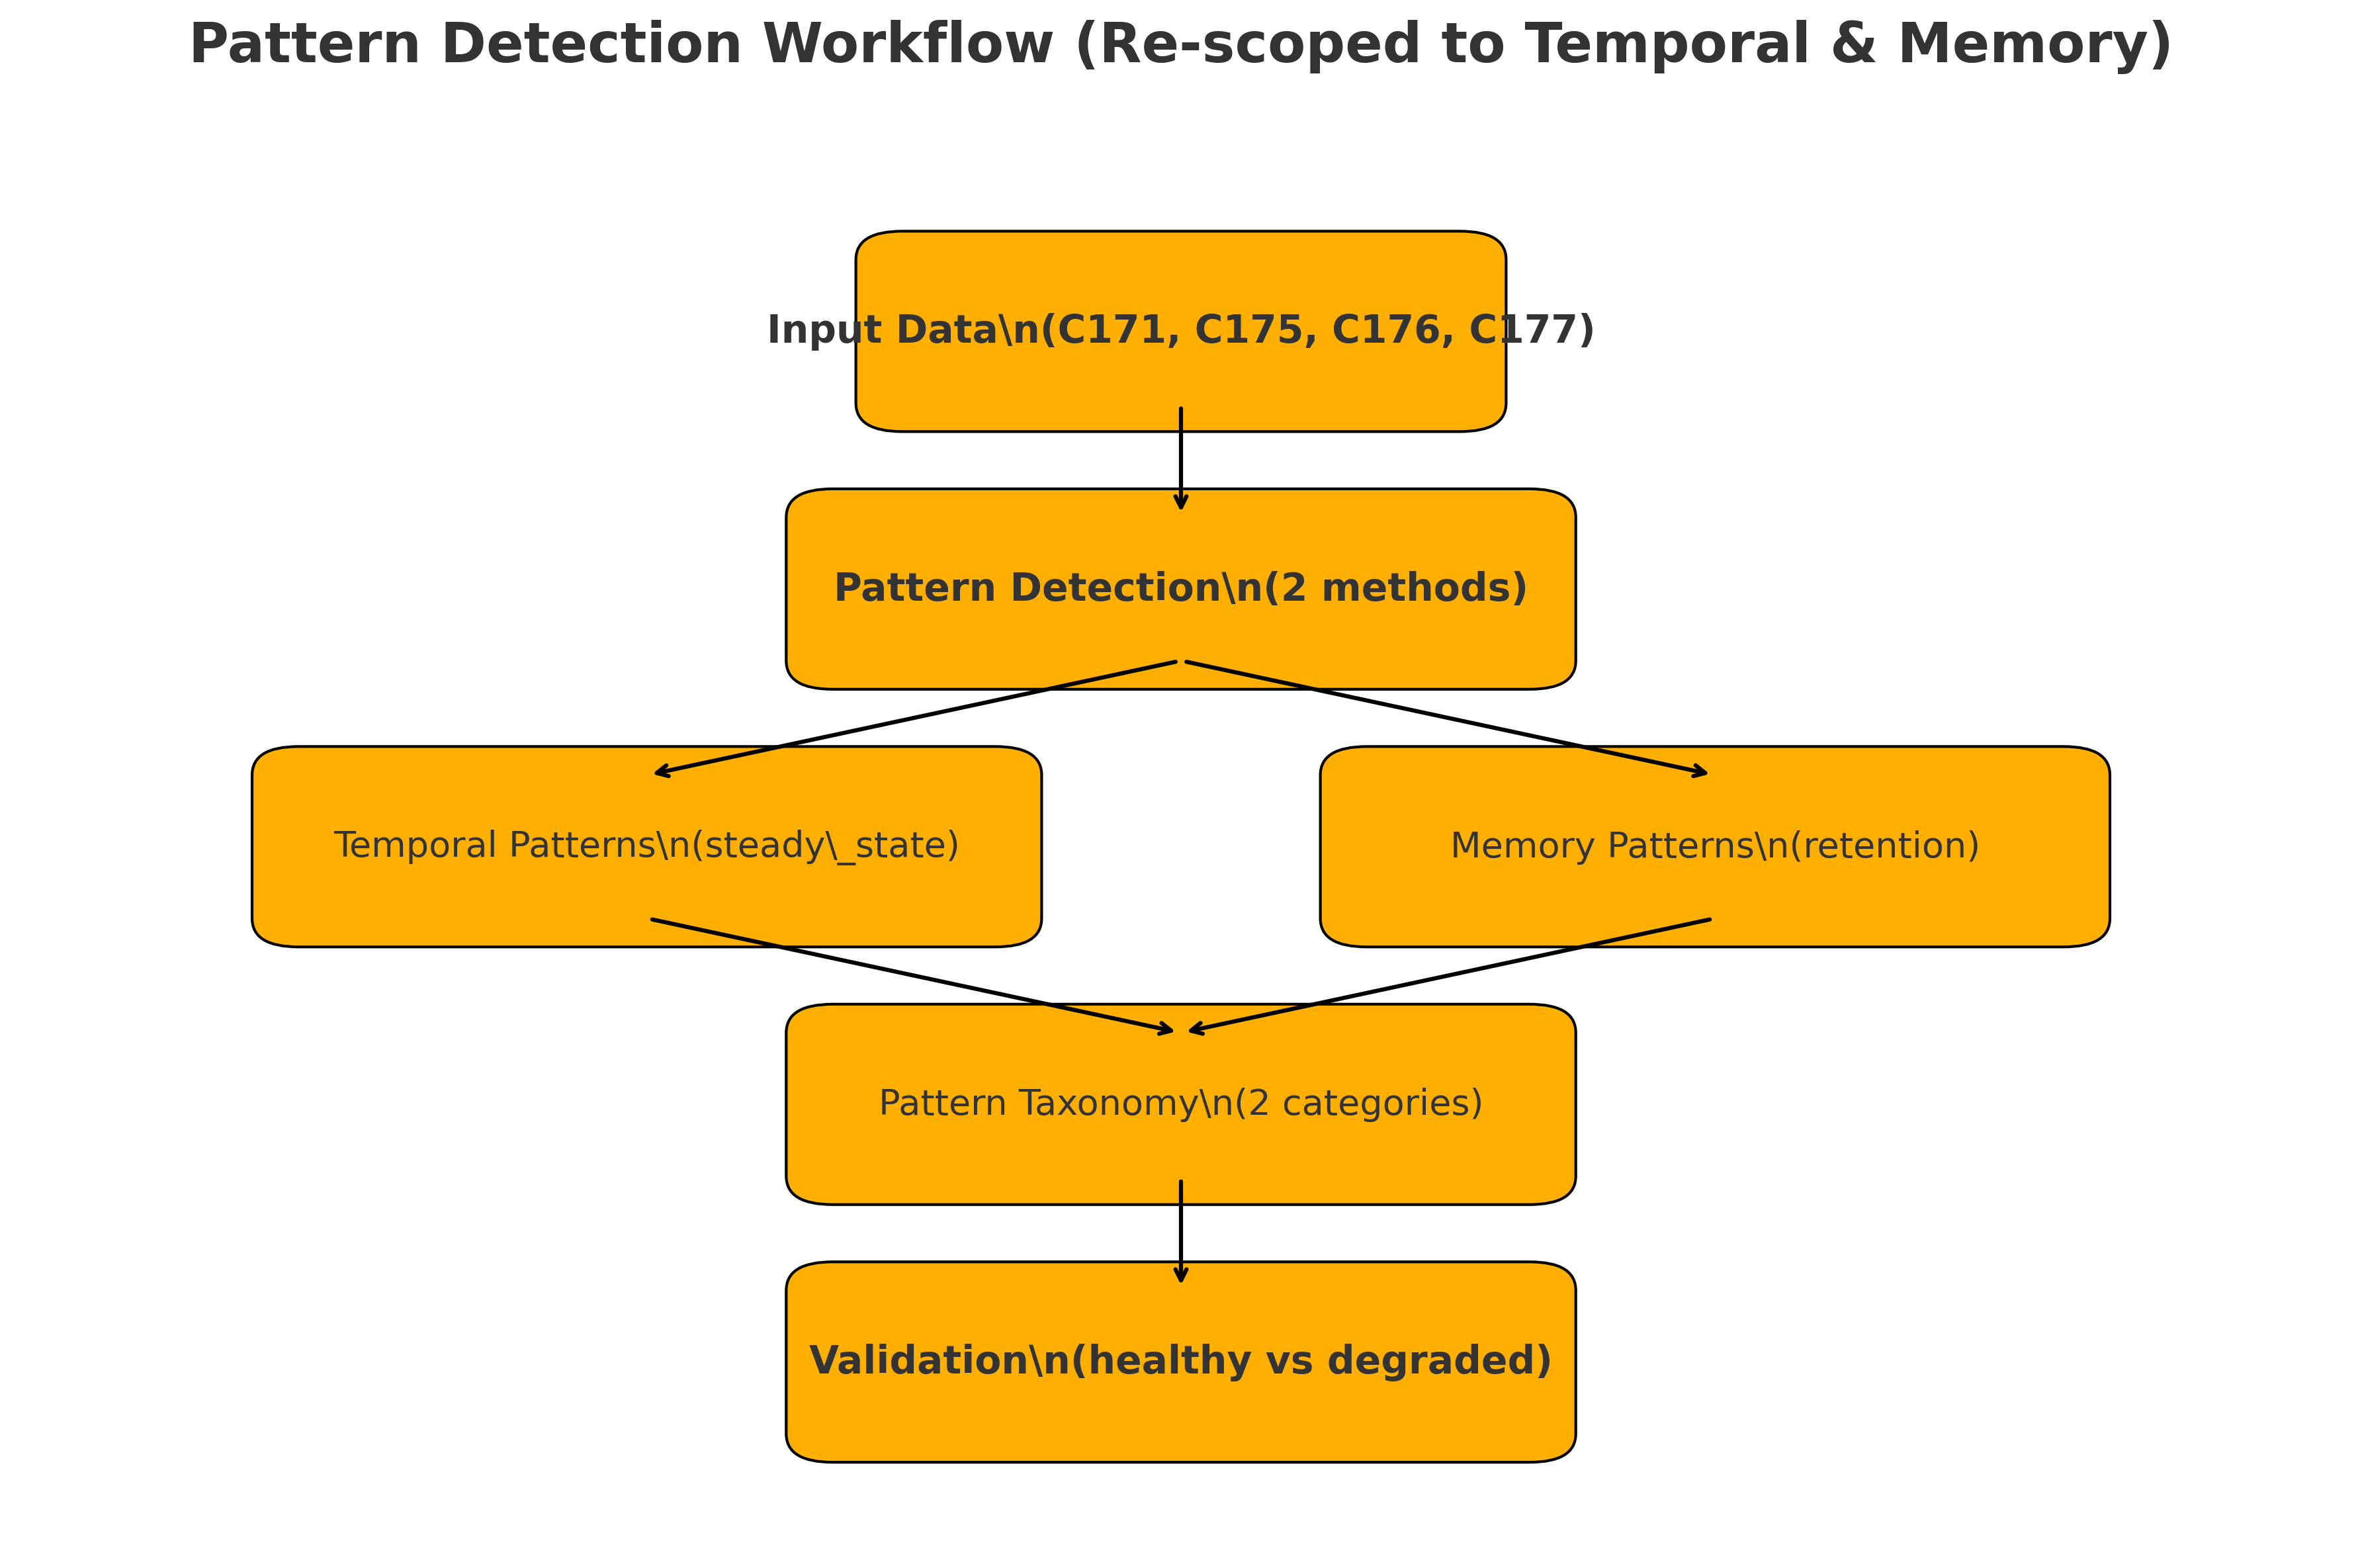
\includegraphics[width=0.9\linewidth]{figure8_pattern_detection_workflow_v2.png}
\caption{Revised workflow re-scoped to two categories.}
\end{figure}

\end{document}
